\chapter{Discussion}
This chapter discusses the findings, and process of the master thesis. Each of the chapters Method, Analysis and results and Evaluation will have a subsection in this chapter. In these sections, challenges faced during the thesis and how they were handled is discussed.

\section{Collection of Wi-fi Traffic}
The selected TP-Link access point had by default enabled Internet group management protocol (IGMP). This function was still enabled during standby traffic capturing, and initial capturing in Oslo environment. During analysis it was identified that if the base filter of frame length greater then 176 bytes was applied, only traffic from the robot vacuum cleaner was presented. This is due to IGMPs use of multicast addressing. The Wireshark output with the base filter is presented in Figure \ref{fig:WLANIGMP_enabled}

\begin{figure}[H]
    \centering
    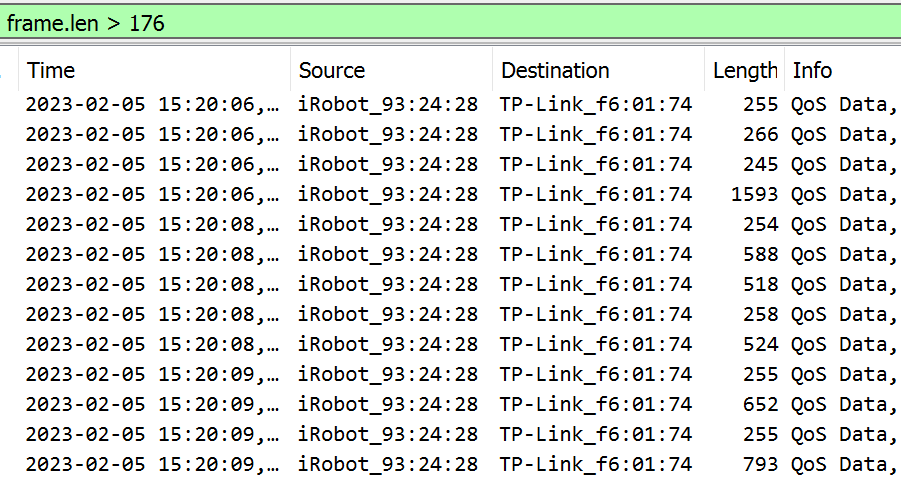
\includegraphics[width=0.8\textwidth]{figures/WLAN_IGMP_enabled.png}
    \caption{Wireshark WLAN capture, included basefilter and enabled IGMP}
    \label{fig:WLANIGMP_enabled}
\end{figure}

The multicast group used by the access point, is not predefined in configuration, but selected by a multicast pool. If the capturing platform should be able to capture this traffic, we would either have to implement IGMP mulitcast discovery, where detected muticast groups would be added to the filter. Or the capture would have to capture all traffic. This includes traffic from other access points in the area. There was conducted a test and captured all traffic from the tp-link access point, but the amount of traffic captured was to large for the Raspberry PI to conduct over time. The filter applied extracted only packets that included either the MAC address of the robot vacuum cleaner (50:14:79:93:24:28) or the multicast group (01:00:5e:7f:ff:fa). As shown in Figure \ref{fig:} traffic from the vacuum cleaner has a destination MAC address for the access point, but the return traffic uses the multicast group as destination address. This IGMP traffic will also include control traffic, which will interfere with the interesting traffic. 

\begin{figure}[H]
    \centering
    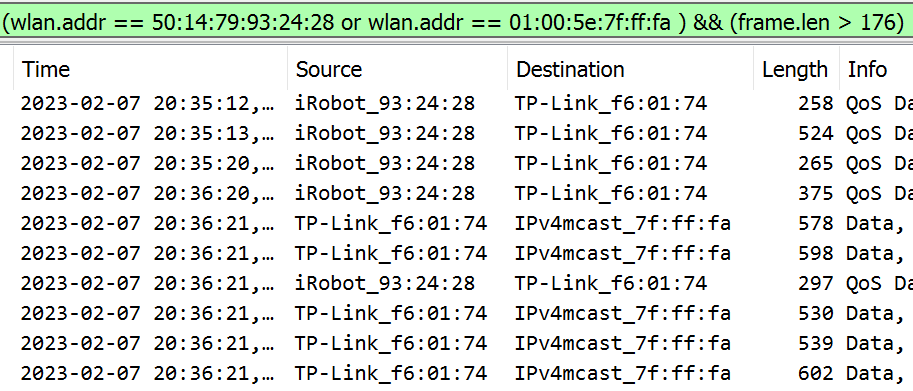
\includegraphics[width=\textwidth]{figures/WLAN_IGMP_ALL.png}
    \caption{Wireshark WLAN capture including IGMP, all SSID traffic}
    \label{fig:WLANIGMP_all_enabled}
\end{figure}

Due to the added complexity of IGMP, it was decided to disable the function. IGMP is not a standard protocol used in wi-fi, the contribution will therefore be valid for all WLANs without IGMP. Another factor is that only one device was connected to the WLAN SSID in the research. If several devices would subscribe to the same IGMP group it would potentially change the traffic flow.

\section{Event triggering}
Event triggering is done in a short time period, this has resulted in that several events has been executed within the same day. This is due to time constrains and availability of the smart home environments. This will not affect the capturing, all events have a separate triggering process in the start of the event. This will be present even if the environments are clean or changed.

A draw back for this type of testing is that the use of time stamps will be conceptual. In normal smart environments these would most likely be triggered at the some day and time and appear more static. A more planned and realistic testing would add value to this research, but the isolated event detection will not be affected. 

\section{Method of Analysis}
Human manually analysis was decided due to the authors knowledge. The complexity and abstraction machine learning would add to the research, could resulted in less ability to evaluate the results. As shown in the evaluation chapter it is still possible to identify signatures and events only with human analysis, the level of complexity and background knowledge is therefore less then for machine learning implementation. The same device selection and test methodology could still be used for machine learning. Machine learning could have create better and more complex signatures, but the results of this research clearly shows that is it possible to detect only with human analysis as well. 

\section{The Complexity of Eavesdropping}
In this thesis the complexity of eavesdropping the different traffic is not addressed. For the wireless traffic an attacker with only need to med in the range of the Wi-Fi access point, but for local LAN they would need physical access to connect their devices. The level of complexity of eavesdropping ISP WAN or core traffic is not consider, this is most likely require a skilled attacker, with a lot resources. 